notes from tuitorial

auto regresive

feed forward cannot learn from the past
recurrent neuron network can learn from the past
xt -> yt 

unrolling through time


Y = activation (Wx +b)


Stored state - memory
internal state html
each neoron has two weight 


basic cell, LSTM cell , GRU cell 

Gradient decent 

back propogation through time

Long Short Term Memory 





confusion matrix
logsoftmax

https://stanford.edu/~shervine/teaching/cs-230/cheatsheet-recurrent-neural-networks


what is softmax?


Product categorization with machine learning is a task that involves automatically assigning products to specific categories or labels based on their features or attributes. It is a common problem in e-commerce, where large catalogs of products need to be organized and classified for various purposes such as search, recommendation, and inventory management.

Machine learning techniques can be employed to tackle product categorization by learning patterns and relationships from labeled training data. Here's a general approach to performing product categorization using machine learning:

Data Collection: Gather a labeled dataset of products, where each product is associated with its corresponding category or label. This dataset serves as the training data for the machine learning model.

Data Preprocessing: Clean and preprocess the product data to remove any irrelevant information, normalize text, handle missing values, and transform the data into a suitable format for the machine learning algorithm. This step may involve techniques such as tokenization, stemming, and removing stop words.

Feature Extraction: Extract relevant features from the product data that can help discriminate between different categories. Features can include textual information (product descriptions, titles), numerical attributes (price, dimensions), and categorical attributes (brand, color).

Model Selection: Choose an appropriate machine learning model for the task of product categorization. Commonly used models include decision trees, random forests, support vector machines (SVM), and neural networks. The choice of the model depends on the complexity of the problem, the size of the dataset, and the available computing resources.

Training: Split the labeled dataset into a training set and a validation set. Use the training set to train the selected machine learning model by feeding it with the labeled product data and their corresponding features. The model learns the patterns and relationships between the features and the categories.

Model Evaluation: Evaluate the trained model's performance using the validation set. Common evaluation metrics for multi-class classification tasks include accuracy, precision, recall, and F1 score. The evaluation helps assess the model's ability to correctly categorize unseen products.

Model Deployment: Once the model has been trained and evaluated satisfactorily, it can be deployed to categorize new, unseen products. The deployed model takes the product features as input and predicts the appropriate category or label for the product.

Iterative Refinement: Product categorization is an iterative process, and the model's performance can be improved by continuously refining the features, trying different machine learning algorithms, and retraining the model with additional labeled data.

It's important to note that the success of product categorization using machine learning heavily depends on the quality and representativeness of the labeled training data, as well as the selection and engineering of relevant features


\begin{table}[h]
    \centering
    \caption{Feature imputation}
    \label{table:feature_imputation}
    \begin{tabular}{ lll }
          \toprule
          
          \textbf{No}& \textbf{Feature} & \textbf{Categorical}\\
          \midrule
          1&Product name & No\\
          3&Description & No\\         
          4&Short description  & No\\
          5&Supplier  & Yes\\
          6&Manufacturer  &  Yes\\           
          7&Price  &  No \\
          8&Dimension  & Yes\\
          \bottomrule
          \end{tabular}
\end{table}


\begin{lstlisting}[language=Python]
    resp=self.es.search("english-name-category",{"_source":["id","name","category"],
    'from':_from,
    'size' :_size ,
    "query": {"match_all": {}}})
\end{lstlisting}


\begin{enumerate}
    \item Euclidean distance.
    % \begin{lstlisting}[language=Python, caption={Euclidean distance formula }]
    %     dist(x, y) = sqrt(dot(x, x) - 2 * dot(x, y) + dot(y, y))
    %         \end{lstlisting}
    \item Manhattan distance.
    \item Hamming distance.
\end{enumerate}


\begin{figure}
    \centering    
    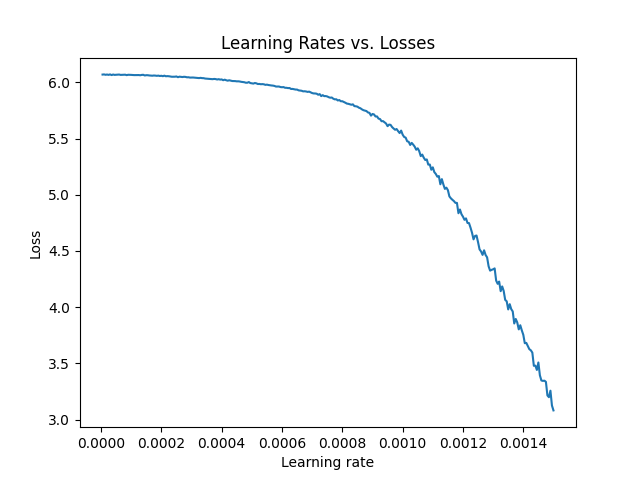
\includegraphics[scale=0.9]{loss_0015.png}
    \caption{Loss vs Learning rate; where $max\_lr = 0.015$}
    \label{fig:Loss value at 0.015}
\end{figure}